\documentclass[parskip=half]{scrartcl}

\usepackage[hidelinks]{hyperref}

\usepackage{amsmath}
\usepackage{amssymb}
\usepackage{amsthm}

\usepackage{pgfplots}
\pgfplotsset{width=20cm,compat=1.18}
\usepgfplotslibrary{external,fillbetween}

\usepackage[dvipsnames,hyperref]{xcolor}

\usepackage{crysymb}

\usepackage{csquotes}
\setquotestyle{british}

\usepackage{fontspec}
\usepackage{unicode-math}
\usepackage{microtype}

\setmainfont{Stix Two Text}
\setmathfont{Stix Two Math}
\setmonofont{Courier}

\usepackage{booktabs}

\begin{document}

\begin{center}
  \textbf{Shamir's secret sharing}
\end{center}

A $(t, n)$-threshold scheme is such that a secret $S$ is split among $n$ participants, and $t$ out of $n$ participants are needed to reconstruct the secret.
Such a scheme provides both security and redundancy since at least, but no more than $t$ parties are required for performing secret-key operations.

Shamir's secret sharing is a simple threshold system used to split a secret into multiple key-shares, and the full secret is reconstructed to perform operations involving the secret.
There exist more complex schemes with additional properties, e.g. distributed key-generation, but we do not consider them here.

A \emph{trusted dealer} picks the secret $S \getsu \ZZ_{\lvert\GG\rvert}$.
The dealer then generates a random polynomial $f$ of degree $t-1$ in the field $\ZZ_{\lvert\GG\rvert}$ such that $f(0)=S$.
We have
\[
  f(x)=S + \sum_{j = 1}^{t-1}a_jx^j,\qquad f(0) = S.
\]
In expanded form,
\[
  f(x) = S + a_1x + a_2x^2 + a_3x^3 + \dots + a_{t-1}x^{t-1}
\]
and clearly $f(0)=S$ which is the secret.
Note that the polynomial is defined in the field $\ZZ_{\lvert\GG\rvert}$ and so computations must be done modulo ${\lvert\GG\rvert}$.

The dealer privately gives each \emph{player} their secret share $s_i=f(i)$, where $i\in\{1,\dots,n\}$, and publishes all $i$.
Notably, $h \gets g^S$, and the public key is not computed from the key-shares.

From Lagrange's interpolation theorem, we know that a polynomial of degree $t-1$ can be reconstructed when knowing at least $t$ points of the polynomial.
Let $f(x_j) = y_j$.
The Lagrange interpolating polynomial is given by
\[
  f(x)=\sum_{j=1}^t y_j \delta_j(x)\quad\text{where}\quad
  \delta_j(x)=\prod_{k=1,k\neq j}^{t}\frac{x-x_k}{x_j-x_k}.
\]

Because we only wish to know $S = f(0)$, we have
\[
  \delta_j(0) = \prod_{k=1,k\neq j}^t \frac{-x_k}{x_j-x_k}\cdot\frac{-1}{-1}=
  \prod_{k=1,k\neq j}^t \frac{x_k}{x_k-x_j}
\]
and so
\[
  f(0)= \sum_{j=1}^{t} y_j\prod_{k=1,k\neq j}^{t}\frac{x_k}{x_k - x_j},
\]
and we can reconstruct the secret.

\textit{Example.}
Let us consider $p = 23$ and $q = (23-1)/2 = 11$.
Let $\GG = \langle2\rangle$ be the group generated by $g=2$ in $\ZZ_{23}$.
We have $\lvert\GG\rvert = q = 11$.

Let $n = 3$ and $t = 2$, meaning that we want to split a secret between $3$ players such that any $2$ players can reconstruct it.
First, let us randomly sample $S \getsu \ZZ_{11}$.
Suppose that we sample $S=4$.
Then, we must randomly sample a single coefficient $a_1 \getsu \ZZ_{11}$ since $t-1 = 1$.
Suppose that we sample $a_1 = 9$.
The polynomial is then given by
\[
  f(x) = S + a_1x = 4 + 9x.
\]

Now that the setup is complete, we can split the secret between $n=3$ parties.
We compute
\begin{alignat*}{2}
  s_1 = f(1) &= (4 + 9) &&\bmod{11} = 2\\
  s_2 = f(2) &= (4 + 18) &&\bmod{11} = 0\\
  s_3 = f(3) &= (4 + 27) &&\bmod{11} = 9
\end{alignat*}
and we privately give $(1, 2)$ to $P_1$, $(2, 0)$ to $P_2$, and $(3, 9)$ to $P_3$.

\begin{figure}[h!]
  \centering
  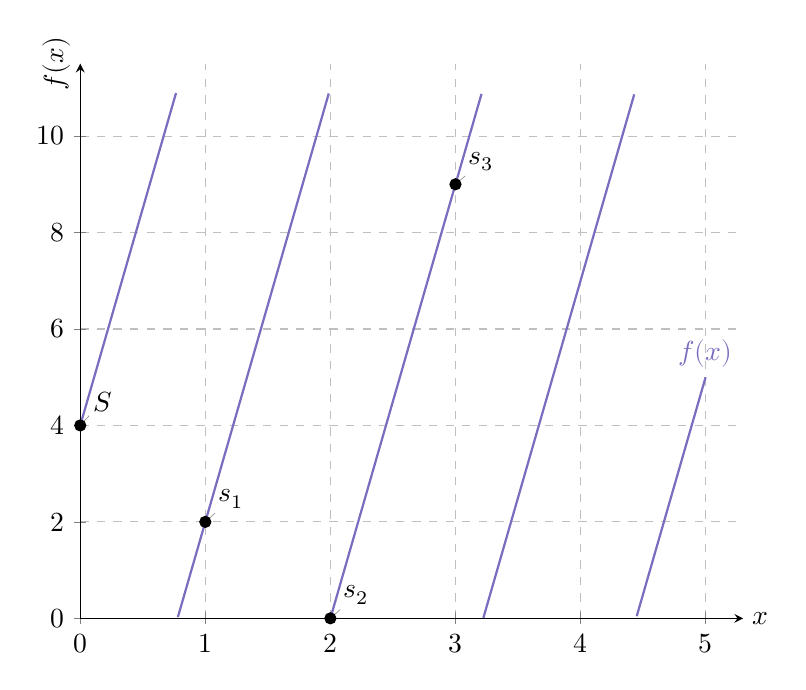
\begin{tikzpicture}
    \begin{axis}[
      width=10cm,
      axis lines = left,
      restrict y to domain=0:10.9,
      grid=major,
      grid style={dashed},
      xlabel=$x$,
      xlabel style={at=(current axis.right of origin), anchor=west},
      ylabel=$f(x)$,
      ylabel style={at=(current axis.above origin), anchor=south},
      domain=0:5,
      xmin=0,ymin=0,
      xmax=5.3,ymax=11.5,
      samples=1000
    ]
      \addplot[thick,Periwinkle] {mod(4 + 9 * x, 11)}
      node[above,pos=1]{$f(x)$};
      \addplot[mark=*] coordinates {(0,4)} node[pin={[pin distance=-1mm]50:{$S$}}]{};
      \addplot[mark=*] coordinates {(1,2)} node[pin={[pin distance=-1mm]50:{$s_1$}}]{};
      \addplot[mark=*] coordinates {(2,0)} node[pin={[pin distance=-1mm]50:{$s_2$}}]{};
      \addplot[mark=*] coordinates {(3,9)} node[pin={[pin distance=-1mm]40:{$s_3$}}]{};
    \end{axis}
  \end{tikzpicture}
  \caption{Graph for $f(x)$ as a continuous function in $\ZZ_{11}$.}
  \label{fig:graph}
\end{figure}

Let us then try reconstructing the polynomial with different subsets:
\begin{enumerate}
  \item $P_1$ and $P_2$
  \[
    f(0) = s_1 \frac{2}{2-1} + s_2 \frac{1}{1-2} =
    2 \cdot 2 + 0 \cdot -1 = 4
  \]
  and we have recovered the secret.

  \item $P_1$ and $P_3$
  
  Notice that here $s_1, s_3$ are not consecutive points, so the indexes in the recovery formula must be readjusted.
  That is, $x_2 = 3$ and not $2$, and $y_2 = s_3$ and not $s_2$.
  \[
    f(0) = s_1 \frac{3}{3-1} + s_3 \frac{1}{1-3} =
    2 \cdot \frac{3}{2} + 9 \cdot -\frac{1}{2} = 3 - 9 \cdot \frac{1}{2}
  \]
  but $1/2$ does not exist in $\ZZ_{11}$.
  Instead, we must find the modular multiplicative inverse of $2$ modulo $11$, i.e. $i$ such that $2i \equiv 1 \pmod{11}$.
  Clearly, $6 \cdot 2 - 2\cdot 11 = 1$ and so the inverse is $6$.

  It follows that
  $f(0) = (3 - 9\cdot 6) \bmod{11} = -51 \bmod{11} = 4$
  and we have recovered the secret.

  \item $P_1$, $P_2$, and $P_3$
  \begin{align*}
    f(0) &= \Biggl[s_1 \frac{2 \cdot 3}{(2-1)(3-1)} + s_2 \frac{1 \cdot 3}{(1-2)(3-2)} + s_3\frac{1 \cdot 2}{(1-3)(2-3)}\Biggr]\bmod{11}\\
    &= (2 \cdot 6/2 + 0 + 9 \cdot 2/2) \bmod{11} = 15 \bmod{11} = 4
  \end{align*}
  and we have recovered the secret.

  \item $P_2$ only
  \[
    f(0) = s_2 \frac{0}{0 - 2} = 0
  \]
  and we have not recovered the secret.
\end{enumerate}

\newpage

\begin{center}
  Demystifying the $\Pi$ notation
\end{center}

How do we interpret $\delta_j(x)=\prod_{k=1,k\neq j}^{t}\frac{x-x_k}{x_j-x_k}$?

More generally, the $\prod_{i = 1}^n a_i$ notation signifies the product of elements $a_1, a_2, \dots, a_n$.
That is,
\[
  \prod_{i = 1}^n a_i = a_1 \cdot a_2 \cdot a_3 \cdot \ldots \cdot a_t.
\]

What if we restrict the values that the iterator $i$ can take?
For example, let $j$ be a value which $i$ cannot take.
Then we have
\[
  \prod_{i = 1, i \neq j}^n a_i = a_1 \cdot a_2 \cdot \ldots \cdot a_{j-1} \cdot a_{j+1} \cdot \ldots \cdot a_t
\]
since we multiply together all values $a_i$ except for $a_j = a_{i = j}$.

In the notation of $\delta_j(x)$, the $j$ in the subscript fixes the value of $j$.
For example, for $\delta_3(x)$, we have $j = 3$.
The $x$ which is given to the function $\delta_j$ is a variable, so its value is fixed by what is passed to the function.
Thus, in the function
\[
  \delta_j(x)=\prod_{k=1,k\neq j}^{t}\frac{x-x_k}{x_j-x_k},
\]
we have that $x, j, t$ are fixed, since $t$ is fixed by the protocol setting.
The only value which then \enquote{changes} when computing $\delta_j(x)$ with a particular input $x$ is the value $k$, since we consider $x_1, x_2, \dots, x_{j-1}, x_{j+1}, \dots, x_t$.
Notice that we have excluded $x_j$.
Indeed, if $j = k$ then $x_k = x_j$ and the denominator is $0$.
Division by $0$ is not defined.

If the reuse of the variable $x$ is confusing, we can also rename it as $x \to z$ to get
\[
  \delta_j(z)=\prod_{k=1,k\neq j}^{t}\frac{z-x_k}{x_j-x_k}.
\]
By unwrapping the product, we get
\[
  \delta_j(z)= \frac{z-x_1}{x_j - x_1} \cdot \frac{z-x_2}{x_j - x_2} \cdot
  \dots
  \cdot \frac{z-x_{j-1}}{x_j - x_{j-1}} \cdot \frac{z-x_{j+1}}{x_j - x_{j+1}} \cdot
  \dots
  \cdot \frac{z-x_t}{x_j - x_t}.
\]

For example, if $z = 0, t = 3$ and $j = 2$ we get
\[
  \delta_2(0) = \frac{0-x_1}{x_2 - x_1} \cdot \frac{0-x_3}{x_2 - x_3} =
  \frac{x_1 \cdot x_3}{(x_2 - x_1)(x_2 - x_3)}.
\]
The values $x_1, x_2, x_3$ are then specific and distinct $x$ coordinates of points on the polynomial.

\end{document}